\begin{spacing}{0.975}
	\chapter{Methods}
	\label{ch:methods}
	
	Building on a physical background, this chapter first introduces generally applicable methods for the translation of an
	injected proton distribution to a hadronic spectrum, which then decays to create neutrinos. Subsequently, the injection
	spectra are described for the previously specified astrophysical settings. To start with, a general case $a \rightarrow b$
	is defined for the reaction. Given a spectrum $dN_a \kern+0.5pt / \kern-0.25pt dE_a$ that describes the number $N_a$ of
	particles $a$ per $E_a$ energy interval, as well as the spectral distribution $F_{a \rightarrow b}$ for the probability
	that particles $b$ are produced by a singular interaction, one can obtain their numbers $N_b$ with respect to their
	energies $E_b$ by solving
	\begin{equation}
		\frac{dN_b}{\raisebox{0.5ex}{$dE_b$}} (E_b) \kern+0.5pt = \kern-1.5pt\int_{\check{E}_a}^{\hat{E}_a} dE_a
		\kern+0.5pt \frac{dN_a}{\raisebox{0.5ex}{$dE_a$}} (E_a) \kern+1.5pt F_{a \rightarrow b} (E_b \kern+0.5pt, \kern-0.5pt E_a)
		\label{eqn:folding}
	\end{equation}
	as the corresponding folding integral. From this formulation, it is clear that both distributions and spectra should be assumed
	to depend on energy, with other arguments such as time $t \kern+0.5pt$ being allowed as well. Additionally, it is always necessary
	to specify $\check{E}_a \leq \hat{E}_a$ as integration bounds, which are usually dictated by kinematic constraints.
	
	To implement and compute all following parametrizations, the \emph{Python} programming language and its library \emph{NumPy}
	are used. Graphical results are generated via the \emph{Matplotlib} package.
	
	
	
	\section{Cross Sections}
	\label{sec:cross}
	
	By defining an effective area perpendicular to the momentum vectors of projectiles and targets, cross sections as described
	in Section \ref{sub:collisions} measure probabilities of collision processes in particle physics and are therefore required
	for the calculation of spectral distributions. Distinctions of particle and antiparticle cross sections vanish at high
	energies and are therefore omitted \cite{pdg}.
	
	
	
	\subsection{Scattering}
	\label{sub:scattering}
	
	\enlargethispage*{2\baselineskip}

	To model total cross sections in hadron-proton scattering, this thesis uses the formula
	\begin{equation}
		\sigma_{hp} = H_h \ln^2 \bigl( s \kern+1.0pt / s_h \bigr) + P_h +
		R_h^1 \bigl( s_h \kern+0.5pt / s \bigr)^{\eta_1} + R_h^2 \bigl( s_h \kern+0.5pt / s \bigr)^{\eta_2}
		\label{eqn:hpr1r2}
	\end{equation}
	as given in \cite{Belousov_2016} for a universal analytic parametrization of the corresponding amplitudes.
	All adjustable parameters are listed in Table~\ref{tab:hadron-scattering} together with relevant meson lifetimes for
	cooling. In this approach, the variable $M$ \kern+0.5pt relates to $H \kern+0.5pt = \pi (\hbar c / M)^2$ and
	$s_h \kern-0.5pt = (m_h + m_p + M)^2$ as an effective mass. Coefficients in \eqref{eqn:hpr1r2} are named after Heisenberg,
	Pomeranchuk and Regge, respectively, and have some qualitative motivation, though the formula itself is mainly a quantitative
	result.
	\newpage
\end{spacing}

\begin{table}[H]
	\centering
	\caption[Fits to the total cross sections in hadron proton collisions.]{Fits to the total inclusive scattering cross sections
			 in hadron proton collisions. Parameters are taken from \cite{Belousov_2016} with $M = \qty{2.121}{\giga\electronvolt}$
			 for $H = \qty{0.272}{\milli\barn}$ as the rate of growth. Both $\eta_1 = \num{0.447}$ and $\eta_2 = \num{0.5486}$ are
			 dimensionless exponents. Rest masses $m_h$ can be found in the particle listings \cite{pdg} and are given in natural units.}
	\label{tab:hadron-scattering}
	\sisetup{group-digits=integer, table-format=2.2}
	\begin{tabular}{c S S S[table-format=1.3] S[table-format=1.3] S}
		\midrule\midrule
		{$h$} & {$P_h \mathbin{/} \unit{\milli\barn}$} &
		{$R_h^1  \mathbin{/} \unit{\milli\barn}$} & {$R_h^2  \mathbin{/} \unit{\milli\barn}$} &
		{$m_h \mathbin{/} \unit{\giga\electronvolt}$} & {$s_h \mathbin{/} \unit{\giga\electronvolt\squared}$} \\
		\midrule
		{$p$} & 34.41 & 13.07 & 7.39 & 0.938 & 15.98 \\
		{$\pi$} & 18.75 & 9.56 & 1.767 & 0.140 & 10.23 \\
		{$K$} & 16.36 & 4.29 & 3.408 & 0.494 & 12.62 \\
		\midrule\midrule
	\end{tabular}
\end{table}


Assuming a quasi universal ratio $\mathscr{R}$ between elastic and total hadron cross sections, one obtains the inelastic
cross section $\sigma_\text{inel} = (1 - \mathscr{R}) \sigma_\text{tot}$ from $\sigma_\text{el} = \mathscr{R} \sigma_\text{tot}$
and $\sigma_\text{el} + \sigma_\text{inel} = \sigma_\text{tot}$ as a unitarity condition. Provided in \cite{Fagundes_2012} is
the model-independent parametrization
\begin{equation}
	\mathscr{R}(s) = \frac{\sigma_{\text{el}\kern+0.5pt} (s)}{\sigma_{\text{tot}\kern+0.5pt} (s)} =
	\mathscr{A} \tanh \bigl( \kern+1.0pt \gamma_1 \kern-1.0pt - \gamma_2 \ln (s) + \gamma_3 \ln^2 (s) \bigr)
	\label{eqn:ratio}
\end{equation}
with a constant asymptote $\mathscr{A}$ at very high energies. Coefficients are given in Table \ref{tab:hadron-ratio} for
different physical settings. Both equations \eqref{eqn:hpr1r2} and \eqref{eqn:ratio} use units of \unit{\giga\electronvolt\squared}
for the $s$  variables. Combining these, Figure \ref{fig:hadron-proton-scattering} depicts the scaling of inelastic cross sections
with energy for different hadrons.

\begin{table}[H]
	\centering
	\vspace{2.0ex}
	\caption[Model independent ratio of elastic and total $\sigma_{h \kern-0.1pt p}$ cross sections.]
			{Almost model independent ratio of hadronic elastic
			 and total scattering cross sections. Factors $\gamma$ are taken from \cite{Fagundes_2012} for varying
			 $\mathscr{A}$ asymptotes.}
	\label{tab:hadron-ratio}
	\sisetup{group-digits=integer, table-format=1.4}
	\begin{tabular}{c S S S[table-format=1.5]}
		\midrule\midrule
		{$\mathscr{A}$} & {$\gamma_1$} & {$\gamma_2$} & {$\gamma_3$} \\
		\midrule
		{$1/2$} & 0.466 & 0.0259 & 0.00177 \\
		{$1$} & 0.2204 & 0.0111 & 0.00076 \\
		\midrule\midrule
	\end{tabular}
\end{table}


Reference \cite{Fagundes_2013} examines the asymptotic rise $\sigma(s) \propto \ln^2(s)$ derived in \cite{Froissart_1961}
as a theoretical upper bound and concludes that it is somewhat exceeded. Additionally, an asymptote $\mathscr{A} = 1/3$ due to
diffraction as opposed to the black disk limit $\mathscr{A} = 1/2 \kern+0.2pt$ from optical theorem predictions is suggested
in \cite{Fagundes_2013}. As parameters are only available in the latter case, all calculations of $\mathscr{R}$
use a ratio \eqref{eqn:ratio} as defined by $\mathscr{A} = 1/2 \kern+0.2pt$ for this thesis. Data matching $\mathscr{A} = 1/3$
imply that $\sigma_{\text{inel}\kern+0.5pt}(s)$ is slightly underestimated, though this is unlikely to
noticeably impact the overall results.

\begin{figure}[H]
	\centering
	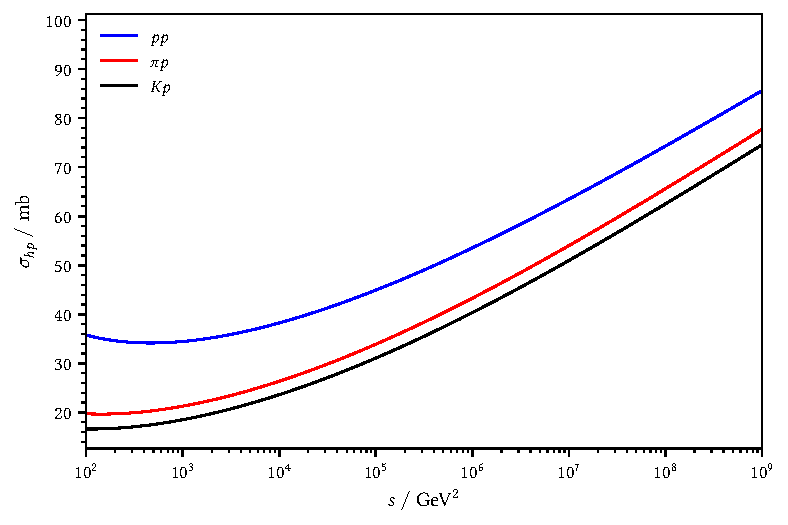
\includegraphics{../plots/build/hadron_proton_scattering.pdf}
	\caption[Inelastic cross sections $\sigma_{h \kern-0.1pt p}$ for hadron-{\kern+0.1pt}proton scattering.]
			{Inelastic cross sections $\sigma_{h \kern-0.1pt p}$ for hadron-{\kern+0.1pt}proton scattering according to the
			 parametrizations \eqref{eqn:hpr1r2} and \eqref{eqn:ratio} reproducing an asymptotic $\cramped{ln^2(s)}$ scaling.}
	\label{fig:hadron-proton-scattering}
\end{figure}




\subsection{Production}
\label{sub:production}

For charm quark production in proton-{\kern+0.1pt}air collisions, reference \cite{Goncalves_2007} gives
\begin{equation}
	x_F \kern+1.0pt \frac{\raisebox{-0.5ex}{$d\sigma$}}{\raisebox{0.5ex}{$dx_F$}} \bigl( x_F \kern+0.5pt, \kern-0.5pt E_p \bigr)
	\kern-0.1pt = a \kern+0.5pt x_F^b \kern+1.0pt \bigl( 1 \kern-0.3pt - x_F^m \kern+0.3pt \bigr)^n
	\label{eqn:charm}
\end{equation}
as the parametrized differential cross section with components
\begin{align*}
	&& a = a_1 \kern-0.5pt \ln\bigl(E_p\bigr) - \kern+0.5pt a_2 \: , && b = b_1 \kern-1.0pt - b_2 \ln\bigl(E_p\bigr) \: , &&
	n = n_1 \kern-1.0pt - \kern+0.5pt n_2 \ln\bigl(E_p\bigr) &&
\end{align*}
for which Table \ref{tab:charm-production} lists all necessary constants. Here, proton energies $E_p$ are defined as viewed
by air nuclei at rest, while the Feynman scaling variable $x_F \kern+1.0pt = p_c \kern+1.5pt / \kern-0.5pt p_s$ specifies
the magnitude ratio of produced charm quark longitudinal momentum to all available momentum in center mass coordinates of the
colliding particles. Application of Section \ref{sub:frames} shows that this approximately fulfills $x_F \kern+1.0pt = x_c$
where $\cramped{x_c = \kern+0.2pt E_c \kern+1.0pt / E_p}$ in the relevant energy ranges. It should be noted that for the values
Table \ref{tab:charm-production} provides, the factor $n_0 \kern-0.5pt = \num{0.075}$ from Table 1 in \cite{Goncalves_2007} 
for the lower energy regime is set to $n_0 \kern-0.5pt = \num{7.5}$ instead, because the parametrization breaks down otherwise.
Further testing reveals another problem with the \qty{e4}{\giga\electronvolt} to \qty{e8}{\giga\electronvolt} region
in that energies of~\qty{26}{\tera\electronvolt}~or lower yield negative differential cross
sections. Considering other approximations made in this thesis, it is therefore decided that an extrapolation from the
\qty{e8}{\giga\electronvolt} to $10^{1 \kern-0.3pt 1} \kern+1.5pt \unit{\giga\electronvolt}$ case to all energies
can be done without producing unreasonably large errors. With these parameters, equation~\eqref{eqn:charm}~only becomes
negative for energies of \qty{140}{\giga\electronvolt} and below.

\begin{table}[H]
	\centering
	\vspace{1.5ex}
	\caption[Parametrization of the $c$ quark differential cross section.]
			{Parametrization of the weighted charm quark
			 production differential cross section. Coefficients are calculated from \cite{Goncalves_2007} to write $E_p$
			 in units of \unit{\giga\electronvolt} without needing redundant conversion steps. The exponent $m = \kern-0.5pt \num{1.2}$
			 is a constant at all energies. For the application at hand, energy ranges beyond the given validity intervals
			 are used as mentioned in the text.}
	\label{tab:charm-production}
	\sisetup{group-digits=integer, table-format=1.3}
	\begin{tabular}{l S[table-format=3.0] S[table-format=4.0] S S S S}
		\midrule\midrule
		{$E_p \mathbin{/} \unit{\giga\electronvolt}$} & {$a_1 \mathbin{/} \unit{\micro\barn}$} &
		{$a_2  \mathbin{/} \unit{\micro\barn}$} & {$b_1$} & {$b_2$} & {$n_1$} & {$n_2$} \\
		\midrule
		{$10^4 - 10^8$} & 826 & 8411 & 0.197 & 0.016 & 8.486 & 0.107 \\
		{$10^8 - 10^{1 \kern-0.3pt 1}$} & 403 & 2002 & 0.237 & 0.023 & 7.639 & 0.102 \\
		\midrule\midrule
	\end{tabular}
\end{table}


Adopting linear scaling with respect to the nucleon number from \cite{Bhattacharya_2015} gives
\begin{equation*}
	\frac{\raisebox{-0.5ex}{$d\sigma$}}{\raisebox{0.5ex}{$dx_c$}} \bigl( x_c \kern+0.5pt, \kern-0.5pt E_p \bigr) = \tilde{A}^{-1}
	\frac{\raisebox{-0.5ex}{$d\sigma$}}{\raisebox{0.5ex}{$dx_F$}} \bigl( x_c \kern+0.5pt, \kern-0.5pt E_p \bigr)
\end{equation*}
for inclusive charm production in proton-{\kern+0.1pt}proton collisions. Approximating air as a gas mixture of roughly \qty{75}{\percent}
nitrogen and \qty{25}{\percent} oxygen, one finds $A = \kern-0.3pt \num{14.5}$ for this factor. By integrating the charmed hadron
cross section defined below and comparing to experimental data in \cite{lhc} for the charm mesons considered in this thesis,
one finds that calculated values exceed measurements~by a factor \num{22.32+-2.34} on average, yielding $\tilde{A} = \num{323.64}$
as a modification to enforce compatibility with observations. One problem of this approach is that \cite{lhc} provides values
at $\sqrt{s \kern+1.0pt} \kern+1.0pt = \qty{13}{\tera\electronvolt}$ or roughly $E_p = \kern+0.1pt \qty{90}{\peta\electronvolt}$ only,
so that deviations at different energies are not accounted for. Similar to earlier reasoning, the resulting inaccuracy is deemed acceptable.

Translation of charm quarks to charmed hadrons is achieved with an integral
\begin{equation}
	\frac{\raisebox{-0.5ex}{$d \kern+1.2pt \tilde{\sigma}$}}{\raisebox{0.5ex}{$dx_h$}}
	\bigl( x_h \kern+0.5pt, \kern-0.5pt E_p \bigr) = \kern-1.0pt \int_{\kern+0.5pt x_h}^1 dz \, z^{-1}
	\frac{\raisebox{-0.5ex}{$d\sigma$}}{\raisebox{0.5ex}{$dx_c$}}
	\bigl( x_c \kern+0.5pt, \kern-0.5pt E_p \bigr) \kern+1.0pt D^{\kern+0.5pt h}_c (z)
	\label{eqn:unmodified}
\end{equation}
where $z = E_h \kern+1.0pt / E_c \kern+0.5pt$ and $x_h = E_h \kern+1.0pt / E_p \kern+0.5pt$ as well as
$x_c = x_h \kern+1.0pt / z$ are fractional energies. Limits for the integration follow from a basic inequality
$E_h \leq E_c \kern+0.2pt \leq E_p$ to incorporate kinematic constraints. Furthermore, the probability
of observing any final state $h$ originating from a $c$ quark is encoded in a \emph{Frag$\kern-0.3pt$mentation Function}
(FF) $D^{\kern+0.5pt h}_c (z)$ dependent on the fraction of hadron to charm energy. Reference
\cite{Metz_2016} addresses the connection between this concept and that of a \emph{Parton Distribution Function}
(PDF) among other things. While a PDF represents the probability density of finding a parton with given momentum inside
a colorless particle, probabilities for color-neutral states existing in individual partons are given by the appropriate
FF instead. The partons described here are either quarks or gluons, which Sections \ref{sub:interactions} and \ref{sub:hadrons}
characterize in more detail.

\newpage

By fitting to existing data or perturbative calculations, models can extrapolate to low momentum fractions that have
not yet been probed experimentally. Such a method has lead \cite{Kniehl_2006} to obtain
\begin{equation}
	D^{\kern+0.5pt h}_{c}(z) = \frac{N_h z \kern+1.0pt (1 - z)^{\kern+0.5pt 2}}
	{\bigl((1 - z)^{\kern+0.5pt 2} + \epsilon_h z \bigl)^{\raisebox{-1.5ex}{$^2$}}}
	\label{eqn:fragmentation}
\end{equation}
with parameters from $\kern+0.5pt e^+e^- \kern-0.8pt$ data in Table \ref{tab:charm-hadrons} as the charm hadron FF used
throughout this thesis. It is important to note that such functions are invariant under charge conjugation, so that there is no
differentiation between quark to particle or antiquark to antiparticle processes.

% \begin{figure}[H]
% 	\centering
% 	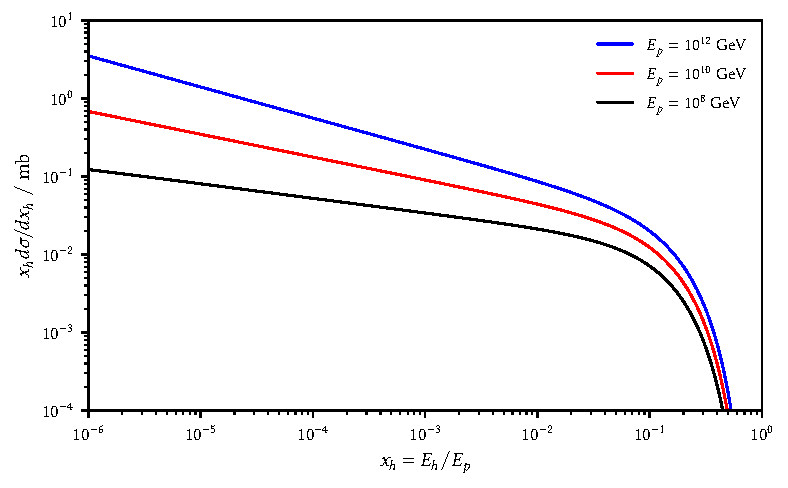
\includegraphics{../plots/build/charm_hadron_cross_section.pdf}
% 	\caption[Inclusive differential cross sections for $\smash{p \kern-0.1pt p \kern+0.6pt \rightarrow D^0 X \kern+0.5pt}$ production.]
% 			{Inclusive differential cross sections for $\smash{p \kern-0.1pt p \kern+0.6pt \rightarrow D^0 X \kern+0.5pt}$ production at
% 			 different proton energies $E_p$ according to the \eqref{eqn:differential} parametrization.}
% 	\label{fig:charm-hadron-cross-section}
% \end{figure}


To account for kinematic constraints, one final modifier has to be included at this point. Because collisions must provide
enough energy for particle formation, charmed hadron energies cannot be lower than their rest masses, leading to
$E_h \geq \kern+0.4pt m_h$ as a natural condition. With Table \ref{tab:charm-hadrons} listing these mass parameters,
a cutoff similar to that in \cite{Kelner_2006} is introduced, rewriting \eqref{eqn:unmodified} to
\begin{equation}
	\frac{\raisebox{-0.5ex}{$d\sigma$}}{\raisebox{0.5ex}{$dx_h$}}
	\bigl( x_h \kern+0.5pt, \kern-0.5pt E_p \bigr) =
	\frac{\raisebox{-0.5ex}{$d \kern+1.2pt \tilde{\sigma}$}}{\raisebox{0.5ex}{$dx_h$}}
	\bigl( x_h \kern+0.5pt, \kern-0.5pt E_p \bigr) 
	\left( 1 - \kern+0.3pt \frac{m_h}{\raisebox{1pt}{$x_h \kern+0.2pt E_p$}} \right)^{\kern-1.0pt 1/2}
	\label{eqn:differential}
\end{equation}
where $E_h \kern-0.3pt = x_h \kern+0.2pt E_p$ ensures physical kinematics are respected. It turns out that this expression
is integrable, whereas the unmodified version \eqref{eqn:differential} is not. Figure \ref{fig:charm-hadron-cross-section}
depicts the $\smash{\cramped{D^0}}$ differential cross section for different incident proton energies and fixed protons as targets.
Comparing this to Figure 7 in \cite{Carpio_2020} indicates similar shapes, though our parametrizations result in less flat
distributions at low $x_h$ values.

\newpage\input{amend/special-head}

\section{Spectral Distributions}
\label{sec:spectral}

Constructing spectra $dN_h \kern+0.5pt / dE_h$ from proton injection requires folding of $F_{p \kern+0.8pt \rightarrow h}$ as
the hadronic distribution for a single $p \kern-0.1pt p \kern+0.9pt$ interaction with the number of protons per energy interval
given by the function $dN_p \kern+0.6pt / dE_p$ obtained from source{\kern+0.1pt}-specific modeling. An analogous approach can
be applied to compute neutrino spectra $dN_\nu \kern+0.6pt / dE_\nu$ from $dN_h \kern+0.5pt / dE_h$ via distributions
$F_{\kern+1.0pt h \kern+0.2pt \rightarrow \nu}$ formulated according to the involved decay modes. Equation \eqref{eqn:folding}
describes exactly this, with the following section providing all required distributions.



\subsection{Charm}
\label{sub:charm}

Spectral distributions for charmed hadron production are calculated according to \cite{Carpio_2020} through
\begin{equation*}
	F_{p \kern+0.8pt \rightarrow h} \bigl( E_h \kern+0.5pt , \kern-0.5pt E_p \bigr) =
	E_p^{\kern+0.5pt -1} \sigma_{p \kern-0.1pt p}^{-1} \bigl( E_p \bigr) \kern+1.0pt
	\frac{\raisebox{-0.5ex}{$d\sigma$}}{\raisebox{0.5ex}{$dx_h$}} \bigl( x_h \kern+0.5pt, \kern-0.5pt E_p \bigr) \: ,
\end{equation*}
with $E_h \kern-0.2pt = x_h E_p$ translating between variables. This can be understood as effectively normalizing term
\eqref{eqn:differential} with respect to the energies and inelastic cross sections of protons, which are scattered as described in
Section \ref{sub:scattering} to yield hadron numbers per unit energy and collision.

To find neutrino spectra from charmed hadrons, the same approach as in \cite{Bhattacharya_2016} is used, which assumes an
effective energy distribution approximated by three{\kern+0.3pt}-body decays for the semileptonic channel to a less massive
pseudoscalar meson. By neglecting lepton masses, one obtains
\begin{equation*}
	\tilde{F}_{\kern+1.0pt h \kern+0.2pt \rightarrow \nu \kern+1.0pt} (y) = D_h^{-1} \kern+1.0pt \Bigl( 6b_ha_h^2 - 4a_h^3
	- 12\lambda_h^2 a_h + 12\lambda_h^2 y - 6b_h y^2 + 4 y^3 + 12 \lambda_h^2 \ln \bigl((1 - y) / \lambda_h \bigr) \Bigr)
\end{equation*}
as a distribution with $y = E_\nu \kern+0.6pt / E_h$ and $F_{\kern+1.0pt h \kern+0.2pt \rightarrow \nu \kern+1.0pt}
\bigl( E_\nu \kern+1.0pt , \kern-0.5pt E_h \bigr) = \mathscr{F}_h \tilde{F}_{\kern+1.0pt h \kern+0.2pt \rightarrow \nu \kern+1.0pt}
(y) / E_h$ for conversion.

Hadron specific coefficients for this equation are defined with the parameter
$\lambda_h = \kern+0.5pt \tilde{s}_h / m_h^2 \kern+0.2pt$ as
\begin{align*}
	a_h = 1 - \lambda_h \: , && b_h = 1 - 2\lambda_h \: , &&
	D_h = 1 - 8 \lambda_h - 12\lambda_h^2 \ln \bigl( \lambda_h \bigr) + 8 \lambda_h^3 - \lambda_h^4
\end{align*}
where both $s_h$ and $m_h$ are listed in Table \ref{tab:charm-hadrons} for all included charmed hadrons. The assumption of
three{\kern+0.3pt}-body decays like $D^+ \kern-2.5pt \rightarrow \kern+1.0pt \overline{\kern-1.5pt K \kern+1.0pt}\kern+1.0pt^0 e^+ \nu_e$
can be justified by consulting \cite{pdg} for information on the relevant particles and comparing branching ratios, which indicate
that purely leptonic modes are strongly suppressed. Hadronic channels such as $D^+ \kern-2.5pt \rightarrow \pi^+ \pi^0$ or
$D^+ \kern-2.5pt \rightarrow K^{\kern+0.5pt -} \pi^+ \pi^+$ are either very improbable as well or occur at significant rates but
do not contribute many high-{\kern+0.2pt}energy neutrinos due to pions and kaons being subject to further cooling before decaying
to leptons. By a similar logic, secondary muon decay is neglected when determining the neutrino spectrum, as muons would experience
additional cooling before decaying and charm cross sections are already low compared to other mesons.

\newpage\input{amend/normal-head}

\begin{spacing}{0.970}
	\begin{table}[H]
	\centering
	\vspace{2.0ex}
	\caption[Coefficients for $c$ hadron production, cooling and decay.]
			{Coefficients for charm hadron production,
			 cooling and decay to neutrinos. All parameters $\epsilon_h$ are taken from leading order QCD fits
			 via the FF as defined and described in \cite{Kniehl_2006} with normalizations $N_h$ given by \cite{Carpio_2020}
			 to rescale the integration of \eqref{eqn:fragmentation} over $[0 \kern+0.5pt , \kern-1.5pt 1]$ to approximately match
			 the fractions $f_h$ provided in \cite{Lisovyi_2016} from measurements. Effective masses $\sqrt{\tilde{s}_h}$ and branching
			 fractions $\mathscr{F}_h$ are determined by \cite{Bugaev_1998} and \cite{Bhattacharya_2016} from fitting decay rates.
			 Mean lifetimes $\tau_h$ and masses $m_h$ are adopted from \cite{pdg} in the particle listings. Mass type
			 quantities use natural units.}
	\label{tab:charm-hadrons}
	\sisetup{group-digits=integer, table-format=1.2}
	\begin{tabular}{c S[table-format=1.4] S[table-format=1.5] S[table-format=4.0] S[table-format=1.3] S S}
		\midrule\midrule
		{$h$} & {$N_h$} & {$\epsilon_h$} & {$\tau_h \mathbin{/} \unit{\femto\second}$} & {$\mathscr{F}_h$} &
		{$\sqrt{\tilde{s}_h} \mathbin{/} \unit{\giga\electronvolt}$} & {$m_h \mathbin{/} \unit{\giga\electronvolt}$} \\
		\midrule
		{$D^{0}$} & 0.577 & 0.101 & 410 & 0.067 & 0.67 & 1.86 \\
		{$D^{+}$} & 0.238 & 0.104 & 1033 & 0.176 & 0.63 & 1.87 \\
		{$D^{+}_{s}$} & 0.0327 & 0.0322 & 501 & 0.065 & 0.84 & 1.97 \\
		{$\Lambda^{\kern-0.5pt +}_{\kern+0.5pt c}$} & 0.0067 & 0.00418 & 203 & 0.045 & 1.27 & 2.29 \\
		\midrule\midrule
	\end{tabular}
\end{table}


	\subsection{Pions \& Kaons}
	\label{sub:pions}
	
	By parametrizing {\textsc{sibyll}}\footnote{
	{\kern+1.5pt}The authors of \cite{Kelner_2006} do not specify the \textsc{sibyll} version that is used.}
	\cite{Fletcher_1994} results, a neutral pion production spectrum of the form
	\begin{equation*}
		\tilde{F}_{p \kern+0.5pt \rightarrow \pi} \kern+1.5pt \bigl( x_\pi \kern+0.7pt , \kern-0.5pt E_p \bigr) = 4\alpha B x_\pi^{\alpha - 1}
		\left( \frac{1 - \kern+0.2pt x_\pi^\alpha}{1 + \kern+0.8pt rx_\pi^\alpha (1 - \kern+0.2pt x_\pi^\alpha \kern+1.0pt )}
		\right)^{\kern-1.0pt 4} \left( ( 1 - \kern+0.2pt x_\pi^\alpha \kern+1.0pt )^{-1} +
		\frac{r (1 - \kern+0.2pt 2x_\pi^\alpha \kern+1.0pt )}{1 + \kern+0.8pt rx_\pi^\alpha (1 - \kern+0.2pt x_\pi^\alpha \kern+1.0pt )}
		\right) \left( 1 - \kern+0.3pt \frac{m_\pi}{\raisebox{1pt}{$x_\pi \kern+1.0pt E_p$}} \right)^{\kern-1.0pt 1/2}
		\label{eqn:pions}
	\end{equation*}
	is found in \cite{Kelner_2006} with $m_\pi = \qty{0.135}{\giga\electronvolt}$ \cite{pdg} translated to natural units and parameters
	\begin{align*}
		&&&& B \kern+0.5pt = \tilde{B} + C \: , &&
		\alpha \kern+0.5pt = \frac{\raisebox{-1.5pt}{$\tilde{\alpha}$}}{\displaystyle\sqrt{C \kern+1.5pt}} \: , &&
		r \kern+1.0pt = \frac{\raisebox{-1.5pt}{$\tilde{r}$}}{\displaystyle\sqrt{C \kern+1.5pt}} &&&&
	\end{align*}
	where a low energy cutoff is enforced via $E_\pi \kern-0.1pt = x_\pi \kern+1.0pt E_p$ in the mass term. From
	\begin{equation*}
		C = c_1 \kern-0.5pt - \kern+0.5pt c_2 \ln \bigl( E_p \bigr) + \kern+0.5pt  c_3 \ln^2 \bigl( E_p \bigr)
	\end{equation*}
	results a dependence on projectile energy for the shape of this distribution.
	
	Coefficients are specified in Table \ref{tab:pion-spectrum} and recalculated from $E_p \kern+0.5pt$ in \unit{\tera\electronvolt}
	to units of \unit{\giga\electronvolt} instead. Under the assumption of a $\smash{\pi^0} \kern-0.5pt$ cross section approximately
	equal to the $\smash{\pi^\pm} \kern-0.5pt$ average and with identical spectra between charged pions, it follows that
	$F_{p \kern+0.5pt \rightarrow \pi} = \tilde{F}_{p \kern+0.5pt \rightarrow \pi} \kern+1.0pt / E_p$ should describe pion
	production regardless of charge reasonably well for the purpose of this thesis.
	
	\enlargethispage*{2\baselineskip}
	\begin{table}[H]
	\centering
	\vspace{2.0ex}
	\caption[Parametrized spectral distribution for pion production.]{Parametrized spectral distribution for
			 neutral pion production. Factors are taken from \cite{Kelner_2006} and converted to write $E_p$
			 in units of \unit{\giga\electronvolt} for $c_k$ coefficients.}
	\label{tab:pion-spectrum}
	\sisetup{group-digits=integer, table-format=1.3}
	\begin{tabular}{S[table-format=1.2] S[table-format=1.2] S[table-format=1.1] S S S}
		\midrule\midrule
		{$\tilde{B}$} & {$\tilde{\alpha}$} & {$\tilde{r}$} & {$c_1$} & {$c_2$} & {$c_3$} \\
		\midrule
		0.25 & 0.98 & 2.6 & 1.515 & 0.206 & 0.075 \\
		\midrule\midrule
	\end{tabular}
\end{table}

	\newpage
\end{spacing}

\begin{spacing}{0.980}
	For a convenient formulation of kaon production, references \cite{Lykasov_2021} and \cite{Lykasov_2022} indicate a constant ratio
	$\pi / K$ at moderately high energies. Similar fractions are retrieved from multiplicities given in \cite{Koers_2006} and lead to
	$F_K \kern+0.5pt / F_\pi = \num{0.12}$ as a simplifying assumption, the validity of which cannot be guaranteed for the application
	at hand. Calculations of kaon spectra still employ this approach but are subject to considerable reservations as a result, because
	fixed ratios to pion spectra are unlikely to be universal. Other than this factor, the pion mass is replaced with that of kaons for
	a correct cutoff in the above expression.
	
	Decays of pions and kaons to neutrinos are approximated via the $h \rightarrow \mu^+ \nu_\mu$ two{\kern+0.2pt}-body channel
	with branching fractions of $\mathscr{F}_{\kern-0.2pt \pi \kern+0.2pt} = \qty{99.99}{\percent}$ and
	$\mathscr{F}_{\kern+0.3pt K \kern+0.2pt} = \qty{63.56}{\percent}$ given in the \cite{pdg}
	particle listings. By decaying, muons produced in these processes can significantly impact the neutrino spectrum. Results from
	\cite{Carpio_2020} suggest that this is particularly relevant for pions. Muonic three{\kern+0.3pt}-body decays of type
	$\mu^- \kern-2.5pt \kern+0.5pt \rightarrow e^- \kern+0.5pt \overline{\kern-0.2pt \nu \kern+0.8pt}_e \nu_\mu$ as well as
	cooling factors depend on the polarization of participating leptons due to the nature of weak force coupling. This complicates
	computations and is thus omitted for the purpose of restricting the present thesis to a manageable scope, though it should be
	remembered as an important caveat for the final results.
	
	The remaining two{\kern+0.2pt}-body decays of ultra-relativistic hadrons $h$ to leptons $l \kern+1.0pt$ obey a distribution
	\begin{equation*}
		F_{\kern+1.0pt h \kern+0.2pt \rightarrow l \kern+1.0pt} \bigl( E_l \kern+0.8pt, \kern-0.2pt E_h \bigr) =
		\mathscr{F}_{\kern+0.2pt h \kern+0.2pt} E_h^{\kern+1.0pt -1} \bigl( 1 \kern-0.3pt - \lambda_h \bigr)^{-1}
	\end{equation*}
	with $m_{\kern+0.5pt \nu} = 0$ and $m_\mu = \qty{0.106}{\giga\electronvolt}$ \cite{pdg} as well as
	$\lambda_h \kern-0.3pt = m_\mu^2 \kern+0.5pt / m_h^2$ as a parameter. This formula is the same whether
	$l = \nu \kern+0.2pt$ or $l = \kern-0.3pt \mu$ because there is one muon for each neutrino. In addition,
	kinematic considerations lead to $E_\mu \kern+0.5pt / E_h > \lambda_h$ and
	$E_{\kern+0.5pt \nu} \kern+0.5pt / E_h < 1 - \lambda_h$ for bounds
	$E_\mu < E_h < E_\mu \kern+0.5pt / \lambda_h$ in case of muons or corresponding limits
	$E_{\kern+0.5pt \nu} \kern+0.5pt / \smash{\bigl( 1 - \lambda_h \bigr)} < E_h < E_p$ when considering neutrinos, which are
	required by \eqref{eqn:folding} for integration.
	
	
	
	\section{Computation}
	\label{sec:computation}
	
	Taking into account previous deliberations, this section now combines these with the contents of Chapter \ref{ch:background}
	to give explicit steps for calculating the results as well as numerical values for the required parameters.
	Additionally, some notes on the implementation are included.
	
	
	\subsection{Injection}
	\label{sub:injection}
	
	The proton spectrum model of young magnetars described in Section \ref{sub:magnetars} starts with an idealized charge density
	$\rho = \omega B_\text{ns} \kern+0.2pt / (2\pi c)$ derived from \cite{Goldreich_1969} and leads to $n = \kern-0.6pt \rho / \kern-0.2pt e$
	for the number of charge carriers. Integrating over the so-called polar caps defined by a radius
	$\smash{R_\text{pc} \kern-1.0pt = \kern-0.2pt R_\text{ns} \sqrt{R_\text{ns} / R_\text{lc}}}$ from which open field lines
	originate and taking a monochromatic energy according to \eqref{eqn:mono} for all times $t \kern+0.5pt$ results
	in a time-derivative delta-functional spectrum
	\begin{equation}
		\frac{d\kern+0.75pt\dot{N}_p}{\raisebox{0.5ex}{$dE_p$}} \bigl( t, E_p \bigr) =
		\frac{B_\text{ns} R_\text{ns}^3 \omega_0^2}{ec \bigl( 1 + \kern+1.5pt t \kern+0.1pt / \kern+0.2pt t_\text{sd} \kern+0.5pt \bigr)}
		\kern+1.0pt \delta \kern+0.5pt \bigl( E_p - E^M(t) \bigr)
		\label{eqn:delta}
	\end{equation}
	that is compatible with a $dN_p \kern+0.5pt / dE_p \propto E_p^{\kern+0.3pt -1}$ power law.
	\enlargethispage*{\baselineskip}\newpage
\end{spacing}

For the AGN setting, a more general DSA scenario like in Section \ref{sub:acceleration} is assumed, yielding
\begin{equation*}
	\frac{dN_p}{\raisebox{0.5ex}{$dE_p$}} \bigl( E_p \bigr) = \mathscr{S} E_p^{\kern+0.2pt -2}
\end{equation*}
with $\kern-0.2pt \mathscr{S} \kern+0.6pt$ for an arbitrary normalization factor that does not need to be specified further,
as this thesis is interested in relative neutrino contributions instead of absolute predictions.



\subsection{Production \& Decay}
\label{sub:decay}

Spectra of hadrons and neutrinos are generally computed as in \eqref{eqn:folding} via folding, though for the hadronic spectrum,
a cooling factor \eqref{eqn:cooling} and optical depth \eqref{eqn:optical} are included, giving
\begin{equation*}
	\frac{dN_h}{\raisebox{0.5ex}{$dE_h$}} \bigl( E_h \bigr) = \mathscr{CO} \int_{E_h}^{\mathscr{E}_{\kern-0.5pt p}}
	\kern-0.5pt dE_p \frac{dN_p}{\raisebox{0.5ex}{$dE_p$}} \bigl( E_p \bigr) \kern+1.5pt
	F_{p \kern+0.8pt \rightarrow h} \bigl( E_h \kern+0.5pt , \kern-0.5pt E_p \bigr)
\end{equation*}
with maximum proton energies $\mathscr{E}_{\kern-0.5pt p}$ as a result. Because the proton spectrum \eqref{eqn:delta}
contains a delta function $\smash{\delta \kern+0.5pt \bigl( E_p - E^M \kern+0.5pt \bigr)}$ in the magnetar case, integration
over $E_p$ simply substitutes $\smash{E^M}$ in place of the proton energy. Accordingly, a limit $\mathscr{E}_{\kern-0.5pt p} = \infty$
can be set to ensure $\smash{E^M} < \mathscr{E}_{\kern-0.5pt p}$ at all times. For the AGN accretion disk, a choice of
$\mathscr{E}_{\kern-0.5pt p} = \smash{\qty{e12}{\giga\electronvolt}}$ is made in accordance with the maximum magnetar proton energy.
A value exceeding that of the GZK cutoff at $E_p = \smash{10^{1 \kern-0.3pt 1}} \kern+1.5pt \unit{\giga\electronvolt}$ described in
Section \ref{sub:cutoff} can be justified by assuming close proximity to the origin of accelerated particles. Proceeding from this,
cross sections and distributions are taken from Sections \ref{sec:cross} and \ref{sec:spectral} to translate the produced hadrons
to neutrinos, which due to their weak interactions mentioned in Section \ref{sub:hadrons} are assumed to be unaffected
by attenuation.

Cooling factors \eqref{eqn:cooling} vary for different hadrons, as $t_\text{dec} \kern-0.5pt = \tau_h E_h / m_h$ and
$t_\text{cool} \kern-0.5pt = \cramped{(\kappa_{h \kern-0.1pt p} \sigma_{h \kern-0.1pt p} n c)^{-1}}$ define the decay and cooling timescales,
with parameters $\tau_h$ and $m_h$ listed in the respective tables, as well as \eqref{eqn:hpr1r2} and \eqref{eqn:ratio} giving the
$\sigma_{h \kern-0.1pt p}$ cross sections, which are approximated to those of kaons for charmed hadrons. The effective optical depth
\eqref{eqn:optical} only describes proton interactions, where the mean free path
$\lambda_{p \kern-0.1pt p} = \cramped{(\kappa_{p \kern-0.1pt p} \sigma_{p \kern-0.1pt p} n)^{-1}}$ and distance $d$ are determined by the
model. Inelasticity factors are assumed to be constants with $\kappa_{h \kern-0.1pt p} = \num{0.8}$ and $\kappa_{p \kern-0.1pt p} = \num{0.5}$
as given in \cite{Carpio_2020}. For the scenario of a newborn magnetar, ejecta properties result in
$n = n_\text{ej}$ \eqref{eqn:number-density} and $d \kern+0.1pt = r_\text{ej}$ \eqref{eqn:ejecta-radius} as parameters. The AGN
accretion disk is modeled by the height parameter \eqref{eqn:height} that varies with radius and characterizes a diffuse density
distribution, as well as the angle $\alpha$ measuring the direction of incidence relative to the disk plane. This is further
simplified by assuming a sharply bound region of height $h$ with homogenous density, leading to $d = h / \kern-2.0pt \sin \alpha$
as the distance travelled by a particle. Because results are insensitive to variations in distance, one can set
$\alpha = \pi \kern+0.25pt / 2$ to find $\sin\alpha = \kern-0.1pt 1$ and $d = h$ with $h = \kern-0.5pt \smash{\qty{e15}{\centi\meter}}$
as stated in \cite{King_2008}. Typical number densities of the order \qty{e15}{\per\centi\meter\cubed} in the disk plane
\cite{Garcia_2013, Garcia_2014} are scaled down to account for the inhomogeneous distribution \eqref{eqn:density} and assumed to be
$n = \kern-0.5pt \smash{\qty{e14}{\per\centi\meter\cubed}}$ for the following calculations. To put this into perspective, typical
SMBH masses of around \qty{e8}{\solarmass} correspond to a \qty{e13}{\centi\meter} Schwarzschild radius. While the radii of accretion disks
can extend to \qty{e18}{\centi\meter} or more, relativistic jets can reach multiple \qty{100}{\kilo\parsec} with terminal bow shocks at
\unit{\mega\parsec} distances from the core \cite{Blandford_2019, King_2008, Murase_2023}.

\newpage

Parameters for the magnetar setting are adopted from \cite{Carpio_2020}. Neutron star radii $R_\text{ns} = \qty{e6}{\centi\meter}$
and masses $M_\text{ns} = \qty{1.4}{\solarmass}$ in accordance with the Chandrasekhar limit that defines the maximum stable mass for
white dwarfs lead to $I_\text{ns} = \qty{e45}{\gram\centi\meter\squared}$ as the classical moment of inertia for a rigid homogenous
sphere, where relativistic effects are ignored and $\qty{1}{\solarmass} = \qty{2e33}{\gram}$ is used. Reference \cite{Haensel_1999}
provides the minimum period of uniform rotation, beyond which the neutron star loses its structural integrity. Choosing twice this
value yields $\omega_0 = \qty{e4}{\per\second}$~as~an~optimistic initial angular frequency. The tilt parameter $\chi$ is set to an
angle of $\chi = \num{0.95}$ radians.~A~magnetic~field of~$B_\text{ns} \kern-0.75pt = \qty{3.2e14}{\gauss}$ leads to a maximum energy
$E^M = \num{5.3} \times 10^{1 \kern-0.3pt 1} \kern+1.5pt \unit{\giga\electronvolt}$ for proton acceleration as well as
$t_\text{sd} = \qty{3.2e3}{\second}$ as the spindown time. With the total ejected mass being similar to that of the
respective progenitor star, values between \qty{10}{\solarmass} and \qty{35}{\solarmass} are possible, from which
the lower bound $M_\text{ej} = \qty{10}{\solarmass}$ is chosen for this scenario. At velocity $\beta_\text{ej} = \num{0.1}$
of the shell, number densities $n_\text{ej} = \smash{\qty{3.1e18}{\per\centi\meter\cubed}}$ are  observed after $t_\text{sd}$
has passed. Lastly, an efficiency $\eta = \num{0.1}$ is assumed for the acceleration of protons.



\subsection{Implementation}
\label{sub:implementation}

In order to calculate neutrino spectra from hadronic distributions, several integrals have to be computed. Discretizing
this computation allows the general case
\begin{align*}
	F(x, y) \kern+1.5pt &= \int_{z_{-}}^{z_{+}} dz \: G(x, z) \, H(z, y) \\
	\intertext{to be rewritten as a Riemann sum. Assuming $G$ and $H$ are integrable over a given interval,}
	F_{ij} \kern+1.8pt &= \sum\nolimits_k D_{kk} \, G_{ik} \, H_{kj}
\end{align*}
converges to the exact solution for sufficiently small subintervals. Transforming variables
\begin{align*}
	&&&& x \rightarrow x_i \: , && y \rightarrow y_j \: , && z \rightarrow z_k &&&&
\end{align*}
and defining $D_{kk} = z_{k+1} \kern-1.0pt - z_k$ leads to the above notation. It is easily shown how this expression in terms of
indices translates to the product of corresponding matrices
\begin{equation*}
	\bm{F} \kern+0.6pt = \bm{G} \, \bm{D} \, \bm{H}
\end{equation*}
as an equivalent formulation. Here, the output $\bm{F} \in \mathbb{R}^{m \times n}$ is obtained from the inputs
$\bm{G} \in \mathbb{R}^{m \times l}$ as well as $\bm{H} \in \mathbb{R}^{l \times n}$ with the square matrix
$\bm{D} \in \mathbb{R}^{l \times l}$ that encodes all step sizes on its diagonal. These results enable a quick and
efficient implementation of the required calculations as program code, where arithmetic array operations can greatly
increase execution speed. Furthermore, logarithmic spacing of $\bm{D}$ often leads to better accuracy after fewer
iterations. To avoid redundant computations, results are stored as data tables.\footnote{
{\kern+1.5pt}For the purpose of reproducibility, all implementations are collected in a dedicated \emph{GitHub} repository:\\
\href{https://github.com/fritzali/bachelor}{github.com/fritzali/bachelor}}



\newpage
\begin{spacing}{0.985}
	\subsection{Event Generation}
	\label{sub:generators}
	
	The description of multiple colliding particle systems constitutes an extremely complex problem, which methods like perturbative
	QF{\kern+0.5pt}T or lattice QCD mentioned in Sections \ref{sub:interactions} and \ref{sub:hadrons} are unable to resolve
	with satisfactory accuracy. Modeling of collider or air shower experiments therefore requires a different approach, realized
	by so-called event generators that fit data in well-tested regions and extrapolate to higher energies via random sampling.
	The Monte Carlo event generator \textsc{sibyll} used as well by \cite{Carpio_2020} and \cite{Kelner_2006} is optimized for
	the simulation of high energy cosmic ray cascades, making it a suitable choice for the calculation of cross sections in an
	astrophysical context such as that of this thesis \cite{Fletcher_1994}.
	
	\begin{figure}[H]
	\centering
	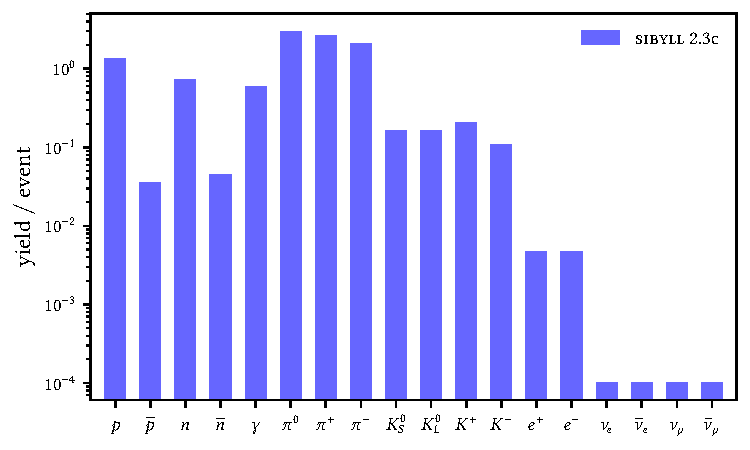
\includegraphics{../plots/build/event_generator.pdf}
	\caption[]
			{}
	\label{fig:event-generator}
\end{figure}

	
	Depicted in Figure \ref{fig:event-generator} are the yields of select particle types per proton-{\kern+0.1pt}proton collision as predicted
	by \textsc{sibyll} 2.3c at $\smash{\sqrt{s \kern+1.0pt} \kern+1.0pt = \qty{1}{\tera\electronvolt}}$ energies. Other particles are
	produced but deemed irrelevant for modeling charm as well as pion and kaon production. This represents one step in the process
	of generating numerical values for the appropriate cross sections. Events are generated at discrete fixed target or center of mass
	energies, with individual yield populations additionally following a separate energy distribution. Accordingly, each bar in
	Figure \ref{fig:event-generator} is an effective integral over all energies of the produced particles. Weighted energy
	differential cross sections $d\sigma \kern+0.5pt / \kern-0.1pt dx$ for specific secondary types can therefore be expressed by a
	histogram in two dimensions, with initial proton energies on one axis and energy of secondaries on the other. Normalizations are
	found by counting the yield and comparing to known values. Creating energy bins at the required resolutions and with sufficient statistics
	is computationally intensive and consumes more time than is available for work on this thesis, which instead uses parametrizations
	as described in the previous sections. Event generator predictions should nevertheless be considered to verify and improve upon the
	following results.
	\enlargethispage*{\baselineskip}\newpage
\end{spacing}
